\documentclass{article}
\usepackage{enumitem}
\usepackage{graphicx}
\usepackage{amsmath}
\usepackage{amssymb}
\usepackage{microtype}
\usepackage{vwcol}  
\usepackage{multicol}
\usepackage{cancel}
\usepackage[top=1cm, left=1.5cm, bottom=0.5cm, right=1.5cm]{geometry}
\usepackage{mathrsfs}
\usepackage{xcolor}
\usepackage{enumitem}
\usepackage{comment}
\usepackage{hyperref}
\usepackage{paracol}
\usepackage{pdfpages}



% Comandos personalizados
\newcommand{\combinat}[2]{\begin{pmatrix} {#1} \\ {#2} \end{pmatrix}}
\newcommand{\magn}[1]{\left[#1 \right]}
\newcommand{\lpn}[1]{\mathscr{L}^{-1}\left\{#1\right\}}
\newcommand{\lp}[1]{\mathscr{L}\left\{#1\right\}}

\newcommand{\frt}[1]{\mathscr{F}\left\{#1\right\}}
\newcommand{\frtn}[1]{\mathscr{F}^{-1}\left\{#1\right\}}

\newcommand{\evalat}[2]{\left. #1 \right|_{{#2}}}
\newcommand{\arccsc}{\operatorname{arccsc}}
\newcommand{\arcsec}{\operatorname{arcsec}}
\newcommand{\arccot}{\operatorname{arccot}}

%    This allows to reference formulas as Section.Subsection. Formula
\newcounter{fmSubSec}[section]
\newcounter{fmCounter}[fmSubSec]
\newcommand{\theformulaCounter}{\arabic{section}.\arabic{fmSubSec}.\arabic{fmCounter}}

\newlist{itemform}{itemize}{1}
\setlist[itemform]{
  label=\textcolor{magenta}{-},
  ref=(\theformulaCounter),
  leftmargin=*,
  noitemsep,
  topsep=0pt,    before=\let\olditem\item\def\item{\stepcounter{fmCounter}\olditem}
}

% Comando para subsecciones (conservando tu nombre)
\newcommand{\fmSubSec}[1]{%
  \stepcounter{fmSubSec}%
  \setcounter{fmCounter}{0}%
  \subsection{#1}%
}

\newenvironment{Figure}
  {\par\medskip\noindent\minipage{\linewidth}}
  {\endminipage\par}
\usepackage{background}

\backgroundsetup{contents=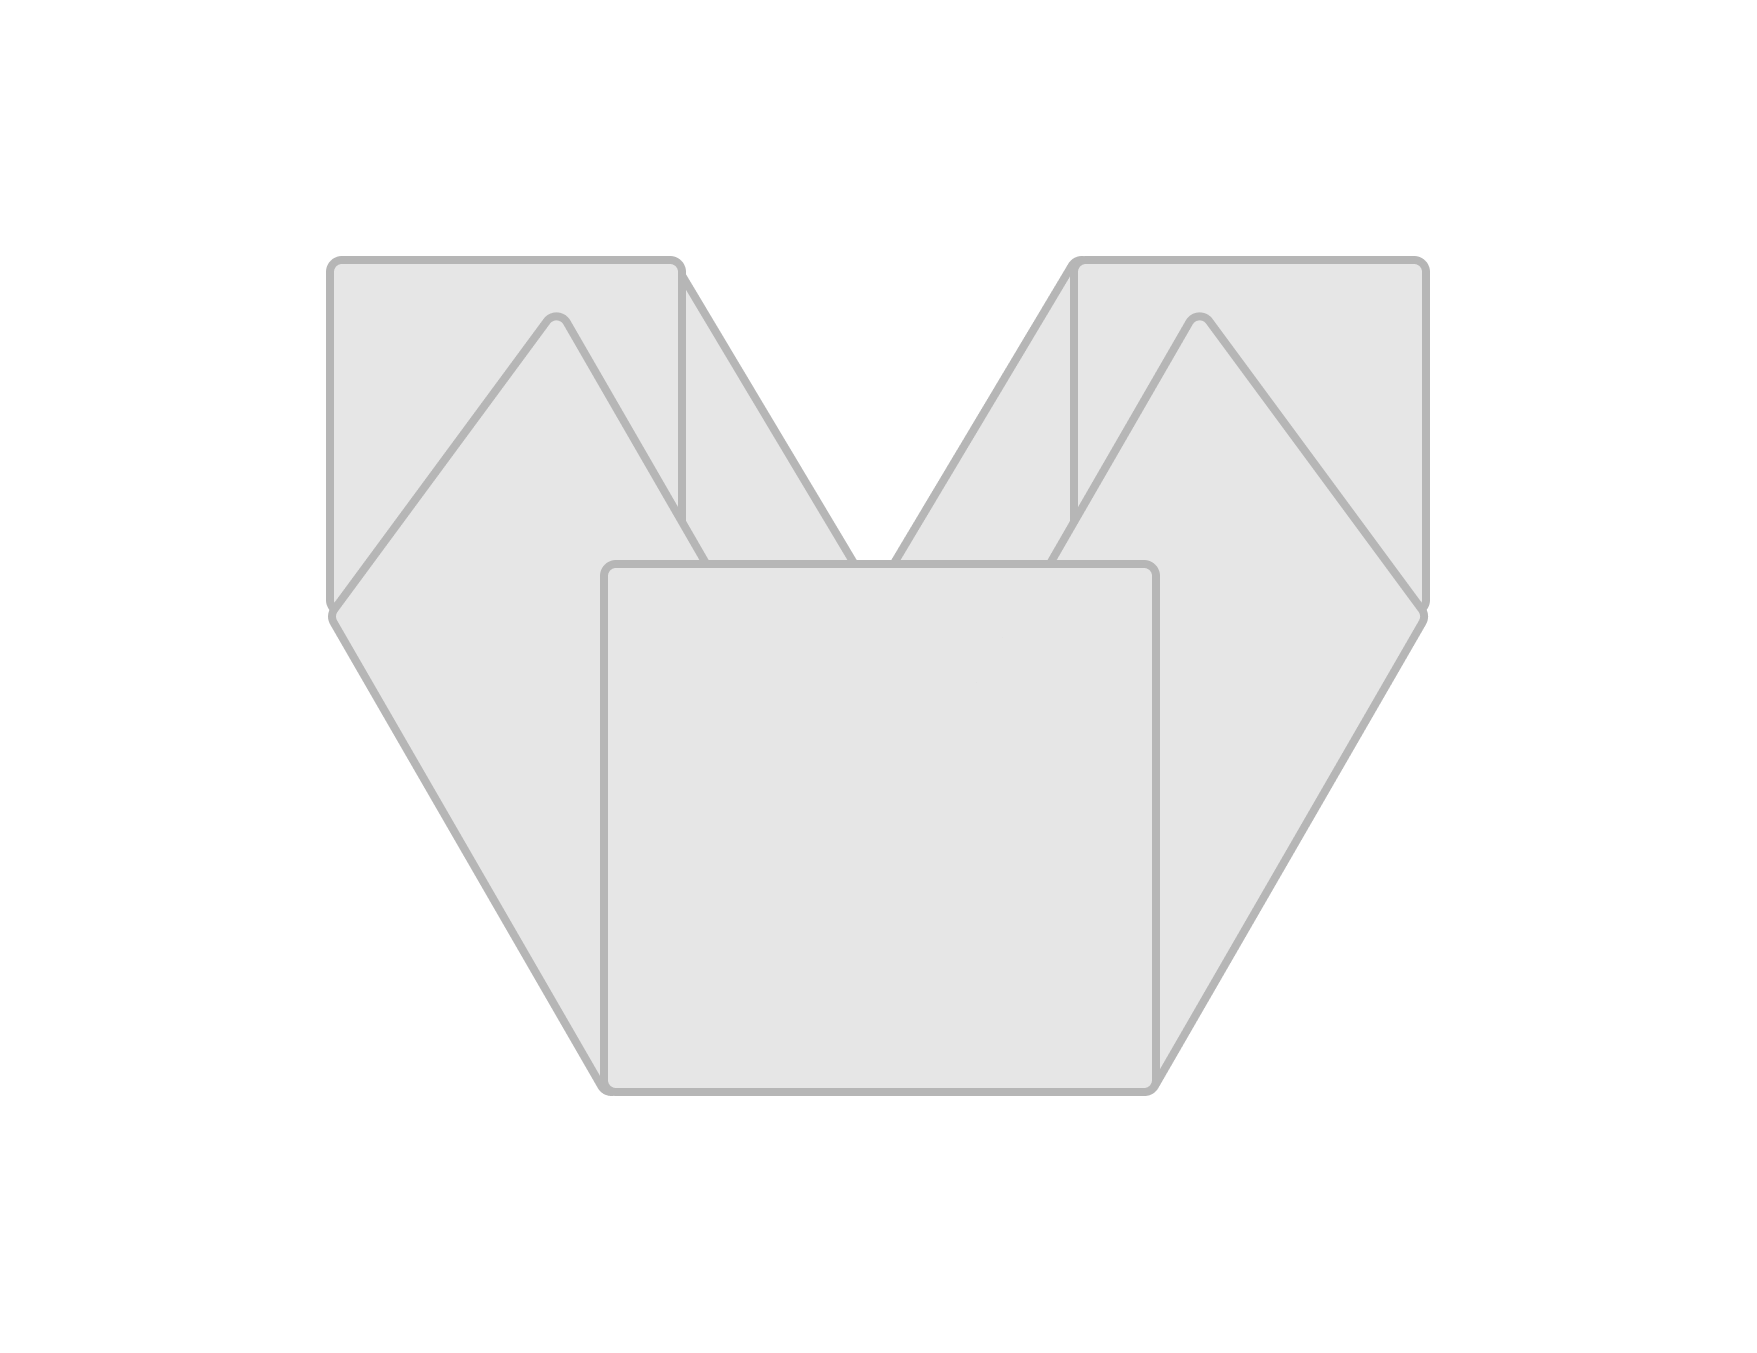
\includegraphics{ALUDAS.png}, scale=1, opacity=0.4,angle =0}

\hypersetup{
    colorlinks=true,
    linkcolor=purple,
    filecolor=magenta,      
    urlcolor=cyan,
    pdftitle={Ultimate Madaf Formulary},
    pdfauthor={Das Reyes},
    bookmarks=true,
    pdfpagemode=FullScreen,
}
\begin{document}
\begin{multicols}{2}

\subsubsection*{Propagación de Errores}
\begin{itemform}
\item \textbf{Regla de potencia} ($f=x_1^{n_1}x_2^{n_2}$), error relativo:
$$\frac{\Delta f}{f} \approx |n_1|\frac{\Delta x_1}{x_1} + |n_2|\frac{\Delta x_2}{x_2}$$
\item \textbf{Peor caso (diferencial exacto)}:
$$\Delta f = \left|\frac{\partial f}{\partial x_1}\right|\Delta x_1 + \left|\frac{\partial f}{\partial x_2}\right|\Delta x_2$$
\item \textbf{Conversión relativo $\to$ absoluto}: $\Delta y = y\dfrac{\Delta y}{y}$
\end{itemform}

\subsubsection*{Tipos de Errores}

\begin{itemform}
    
\item \textbf{Error absoluto, relativo, y relativo porcentual}
\[
e=x_{\mathrm{medido}}-x_{\mathrm{ref}}
\quad e_r=
\frac{e}
{x_{\mathrm{ref}}}
\quad e_{\%}=\frac{e}{x_{\mathrm{ref}}}\times100
\]


\item \textbf{Error maximo permitido}

Para un instrumento con spec de $\pm a\%\text{ de lectura}\pm b$


El error máximo permitido puede expresarse como:

\[
E_{\max}
=
\frac{a}{100}|x|+b
\]

\item  \textbf{Error absoluto por \%FS}


Si la exactitud está especificada como: \(
\pm a\%FS
\)

El error absoluto máximo es:

\[
E_{\max}
=
\frac{a}{100}FS
\]

\item \textbf{Bias}:
Sesgo $$
Bias= \bar{x}-x_{\text{ref}} \quad Bias_{\%}=\frac{Bias}{x_{\text{ref}}}\times100
$$
\item \textbf{Error de no linealidad/ Histeresis}:

$$
e_{NL,i}=\max|y_i-y_{\text{recta},i}|
\quad
e_{NL,\%}=\frac{e_{NL,max}}{FS}\times100
$$
\end{itemform}




\begin{itemform}
\item \textbf{Media} y \textbf{desviación estándar muestral}:
$$\bar{x}=\frac{\sum x_i}{N} \quad \sigma=\sqrt{\frac{\sum(x_i-\bar{x})^2}{N-1}}$$
\end{itemform}

\subsubsection*{Regresión Lineal (Mínimos Cuadrados)}
\begin{itemform}
\item \textbf{Ajuste} $y=ax+b$:
$$a=\frac{N\sum xy-\sum x\sum y}{N\sum x^2-(\sum x)^2} \quad b=\bar{y}-a\bar{x}$$
\item \textbf{Coeficiente de determinación}:
$$R^2=1-\frac{\sum(y_i-\hat{y}_i)^2}{\sum(y_i-\bar{y})^2}$$
\end{itemform}


\subsubsection*{SNR y Ganancia}
\begin{itemform}
\item \textbf{Relación senal/ruido}:
$$SNR_{dB}=20\log_{10}\left(\frac{V_{senal}}{V_{ruido}}\right)$$
\item \textbf{Ganancia de etapas en Cascada}
$$
G_T = G_1G_2\cdots G_n \quad G_{T,dB}=G_{1,dB}+G_{2,dB}+\cdots+G_{n,dB}$$
\end{itemform}

\subsubsection*{Clasificación de Errores}
\begin{itemform}
\item \textbf{Grueso (equivocación)}: 

falla de operador, ej. rango/escala mal seleccionada; no es reproducible por diseño del equipo.
Si $|\Delta x|>3 \sigma$, investigar causa asignable.

\item \textbf{Sistemático}:

reproducible y determinista (offset, ganancia, no linealidad, deriva, interferencia periódica como 60\,Hz).
\item \textbf{Aleatorio}:

dispersión estocástica de causa no asignable; se reduce promediando repeticiones.
\end{itemform}

\subsubsection*{Offset, Ganancia y Combinaciones}
\begin{itemform}
\item \textbf{Offset puro} ($y=x+b$):

error $=$ constante en todo el rango (desplazamiento aditivo con entrada cero).
\item \textbf{Ganancia pura} ($y=ax$, $a\neq1$): 

error crece proporcional a la entrada (pendiente $\neq 1$).

\item \textbf{Recta de corrección} ($T_{real}=aT_{ind}+b$):

$a\neq1 \Rightarrow$ error de ganancia; $b\neq0 \Rightarrow$ error de offset.
\end{itemform}

\subsubsection*{Precision, Exactitud y Veracidad}
\begin{itemform}
\item \textbf{Precisión}: dispersión de mediciones repetidas (e. random).
\item \textbf{Veracidad}: cercanía a valor verdadero (error sistemático).
\item \textbf{Exactitud}: cercanía a valor verdadero y dispersión pequeña (combinación de exactitud y precisión).

\end{itemform}

\subsubsection*{Zona Muerta, Histéresis y Umbral}
\begin{itemform}
\item \textbf{Umbral}: mínimo estímulo absoluto desde reposo (cero) que produce respuesta.
\item \textbf{Resolución}: mínimo incremento detectable en cualquier punto del rango.
\item \textbf{Zona muerta}: rango de entrada donde la salida es nula.
\item \textbf{Histéresis}: salida distinta según sentido de variación, no corregible con offset/ganancia estáticos .
\item \textbf{Saturación}: si $|V_{out,ideal}|>|V_{out,max}|$, la salida se recorta al límite físico.
\end{itemform}




\subsubsection*{Repetitividad y Reproducibilidad}
\begin{itemform}
\item \textbf{Límite de repetitividad}: $r=2.8\,s_r$; si $|\Delta x|>r$, investigar causa asignable.
\item \textbf{Diagnóstico}: $\dfrac{s_R}{s_r}\gg1 \Rightarrow$ R Reproducibilidad, r Repetitividad
\end{itemform}


\begin{itemform}
\item \textbf{Intervalo máximo de calibración}:
$$t_{cal}=\frac{\%FS_{tolerable}}{\text{Deriva}\ (\%FS/\text{ano})}$$
\end{itemform}



\subsubsection*{Resolución del ADC}
\begin{itemform}
\item \textbf{Niveles de un ADC de $N$ bits}: $L=2^N$
\item \textbf{Niveles requeridos}:
$$N_{niveles}=\frac{\text{Rango}}{\text{Resolución deseada}}$$
\item \textbf{Bits mínimos}:
$$
N \ge \log_2\left(\frac{FS}{\Delta_{max}}\right)
$$

\end{itemform}

\end{multicols}


\end{document}